\documentclass[handout,10pt]{beamer}
\usepackage{pgfpages}
\pdfpkresolution=8000

% Coins arrondis
%\pgfpagesuselayout{rounded corners}[corner width=2pt]

% 2 vignettes par pages avec les notes
%\usepackage{handoutWithNotes}
%\pgfpagesuselayout{2 on 1 with notes landscape}[a4paper,border shrink=5mm]

% 2 vignettes par pages sans les notes
%\pgfpagesuselayout{2 on 1}[a4paper,border shrink=5mm]

% Pour obtenir la présentation au format d'un article.
%\documentclass[a4paper]{article}
%\usepackage{beamerarticle}
%\usepackage{pgf}
%\mode<article>{\usepackage{fullpage}}

% Présentation en mode normal et démarrage en plein écran.
%\documentclass[{pdfpagemode=FullScreen,colorlinks=false}]{beamer}
%\mode<presentation>

% Thèmes prédéfinis (sauf Evry qui nécessite le .sty associé).
%\usetheme{PaloAlto}
%\usetheme{Darmstadt}
\usetheme{Evry}

% Les paquets classiques français pour éviter les problèmes d'accents
% Ne pas oublier d'enregistrer le fichier au format UTF8
\usepackage[francais]{babel} % pour les cesures : cf. frenchb2-doc.pdf (doc babel)
\usepackage[utf8]{inputenc}  % le fichier doit être sauvegardé en utf8
\usepackage[T1]{fontenc}     % Encodage des fontes
\usepackage{eurosym}
\usepackage{verbatim}
\usepackage{color}
\usepackage{amsmath}


\title{Unix/Linux : Guide de survie à la ligne de commande}
\author{Olivier DELHOMME}
\date{2015}

\begin{document}

\normalfont\normalfont

\frame
{
    \titlepage
    \begin{center}
    \end{center}
}


\section{Définitions}
\frame
{
    \frametitle{Conventions}

    \begin{itemize}
        \item {\ttfamily <<~dup~>>, <<~delhomme~>>, <<~admin~>>} font référence à des utilisateurs,
        \item {\ttfamily <<~monfichier~>>, <<~monautrefichier~>>} font référence à des noms de fichiers,
        \item {\ttfamily <<~mondossier~>>, <<~monautredossier~>>} font référence à des noms de dossiers.
    \end{itemize}
}


\section{Historique}
\frame
{
    \frametitle{Quelques dates}

     \begin{itemize}
        \item Années 60 : création de MULTICS,
        \item 1969 Création de UNICS (AT\&T),
        \item 1970 Création d'UNIX (en assembleur pour PDP11),
        \item 1972 Ré-écriture en C (domaine public grâce à un décret anti-trust sur AT\&T),
        \item 1980 --> diffusion dans toutes les universités,
        \item 1983 Publication du system V et levée du décret : UNIX est vendu par AT\&T,
        \item 1991 Sortie de GNU/Linux 0.0.1,
        \item 1993 Tous les unix sont basés sur System V,
        \item 2002 Mac OS X (dont le coeur est un BSD),
        \item 2012 Unix a 42 ans (101010),
        \item 2012 GNU/Linux a 21 ans.
    \end{itemize}
}


\frame
{
    \frametitle{Arbre généalogique}

    \begin{center}
        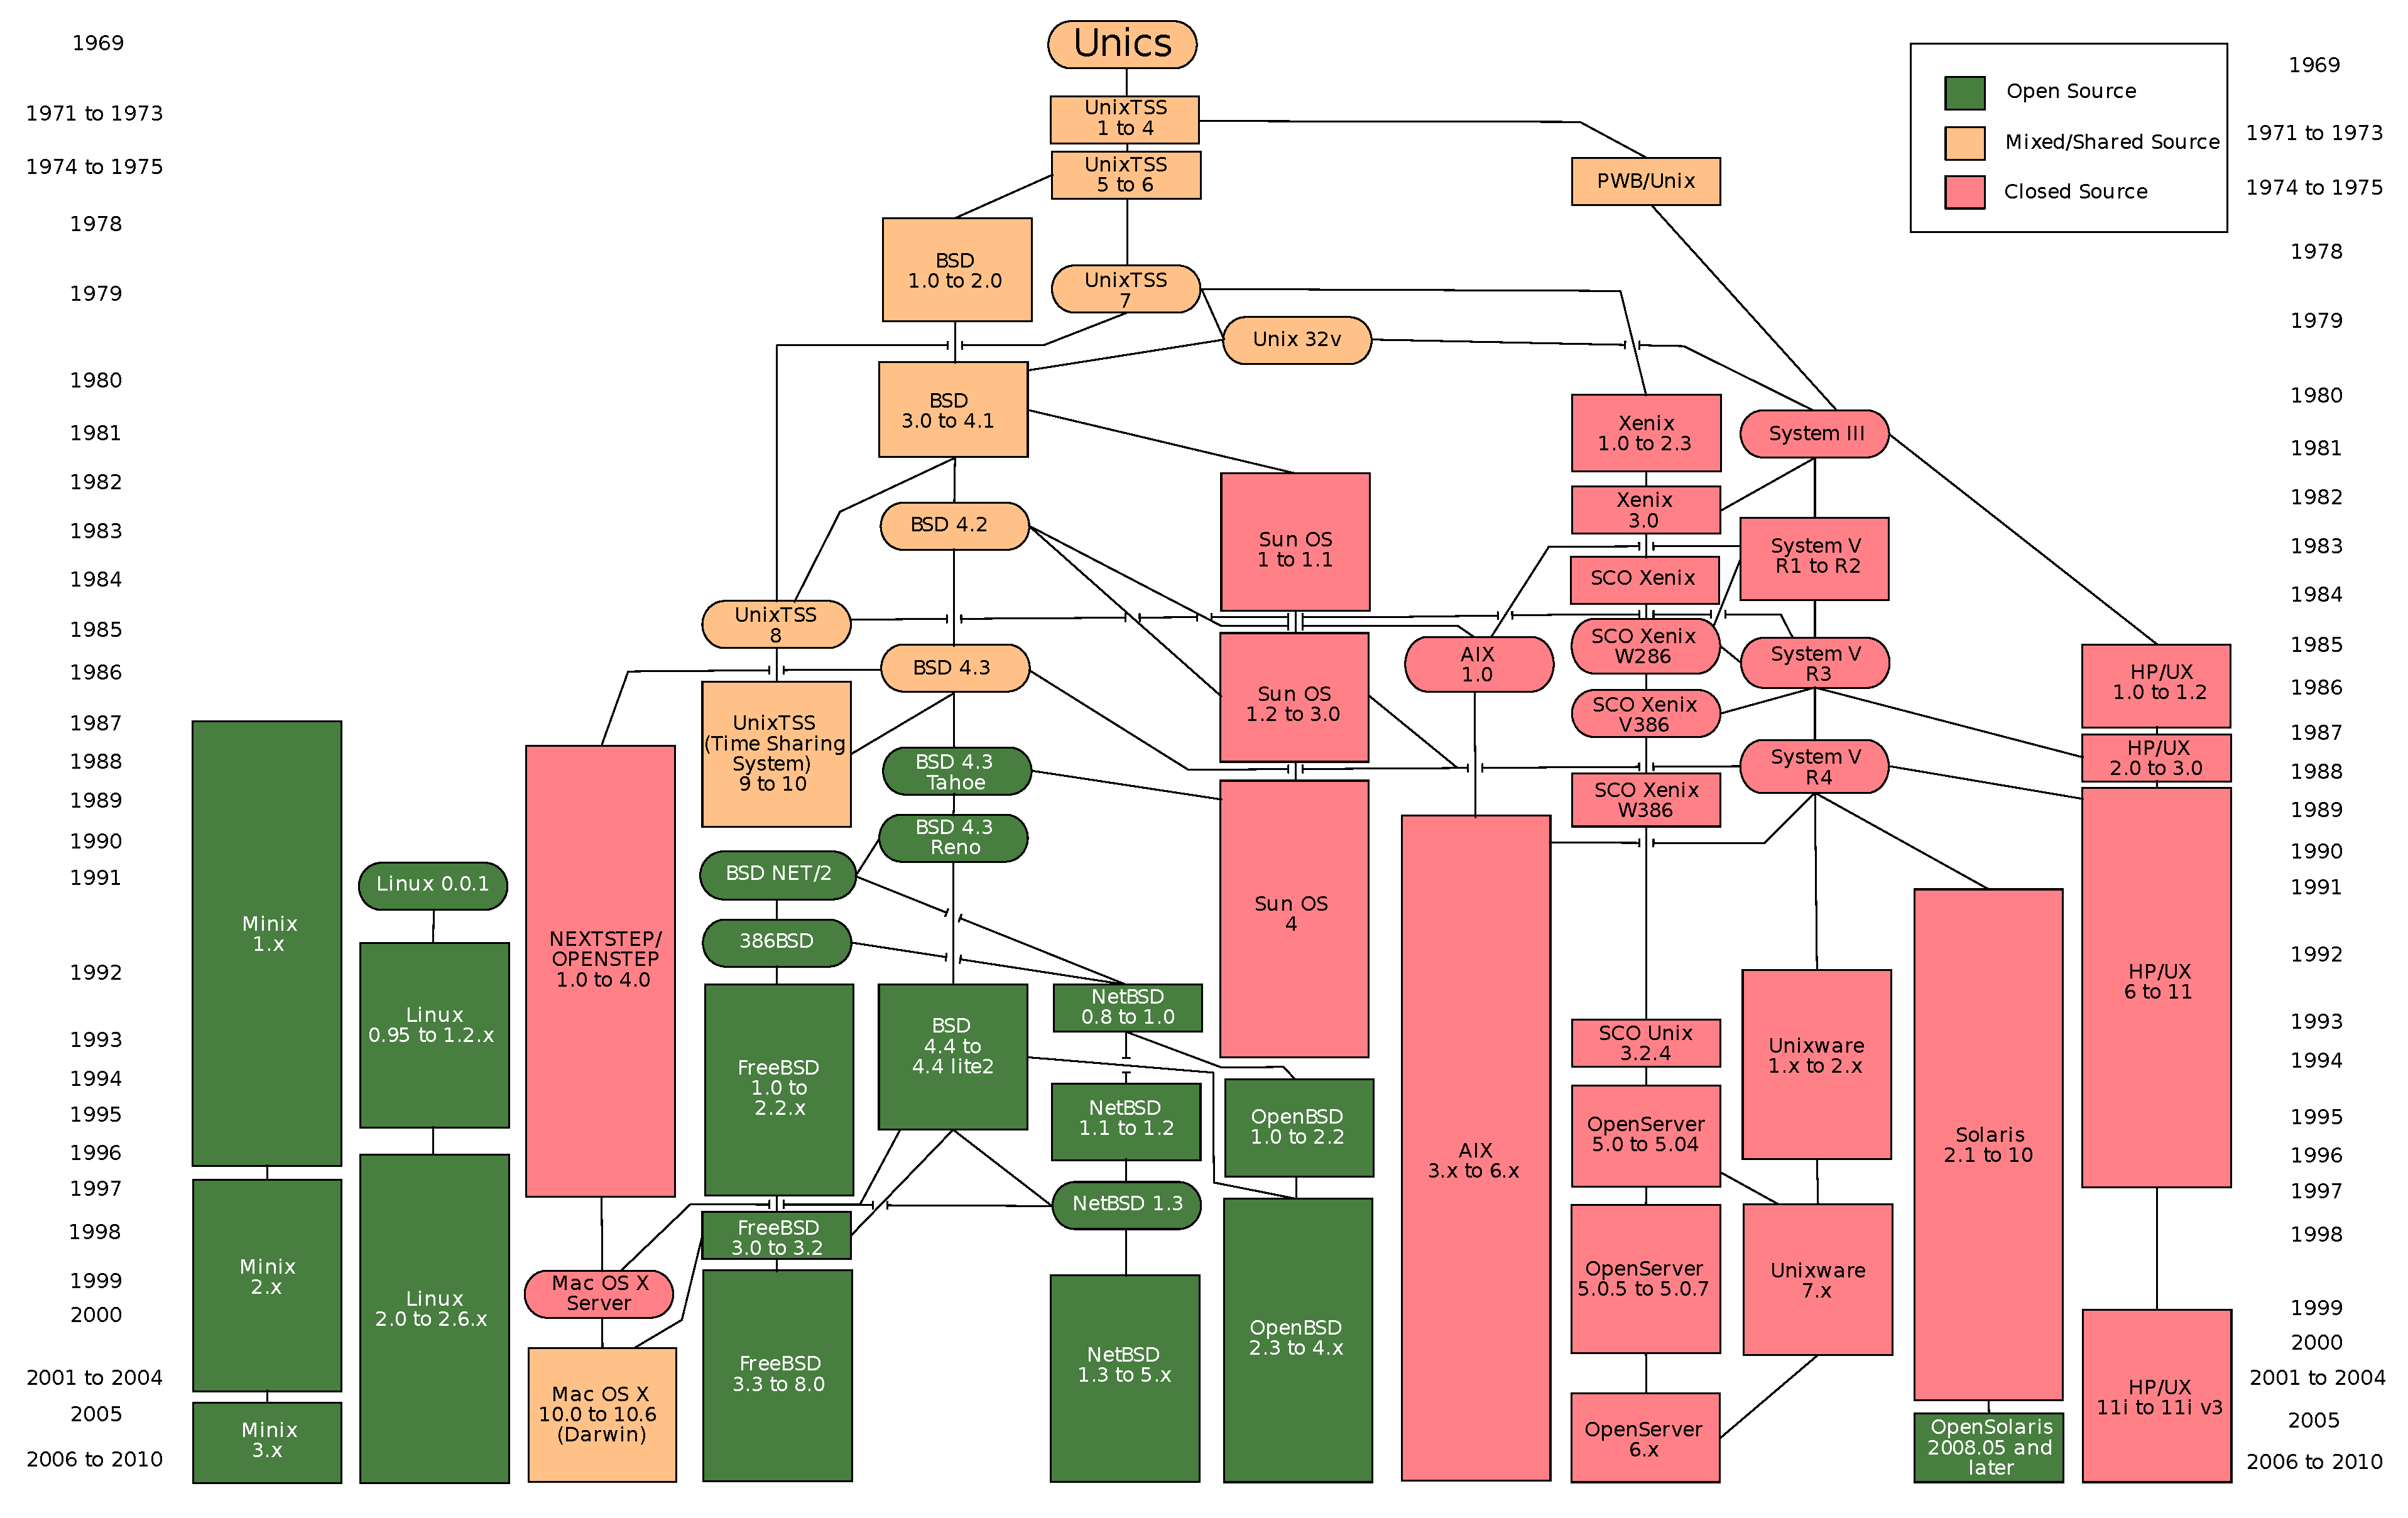
\includegraphics[width=10.5cm]{images/Unix_history-simple.pdf}
    \end{center}
}


\section{Environnement de travail}
\frame
{
    \frametitle{Quel environnement aujourd'hui}

     \begin{center}

        \begin{figure}
            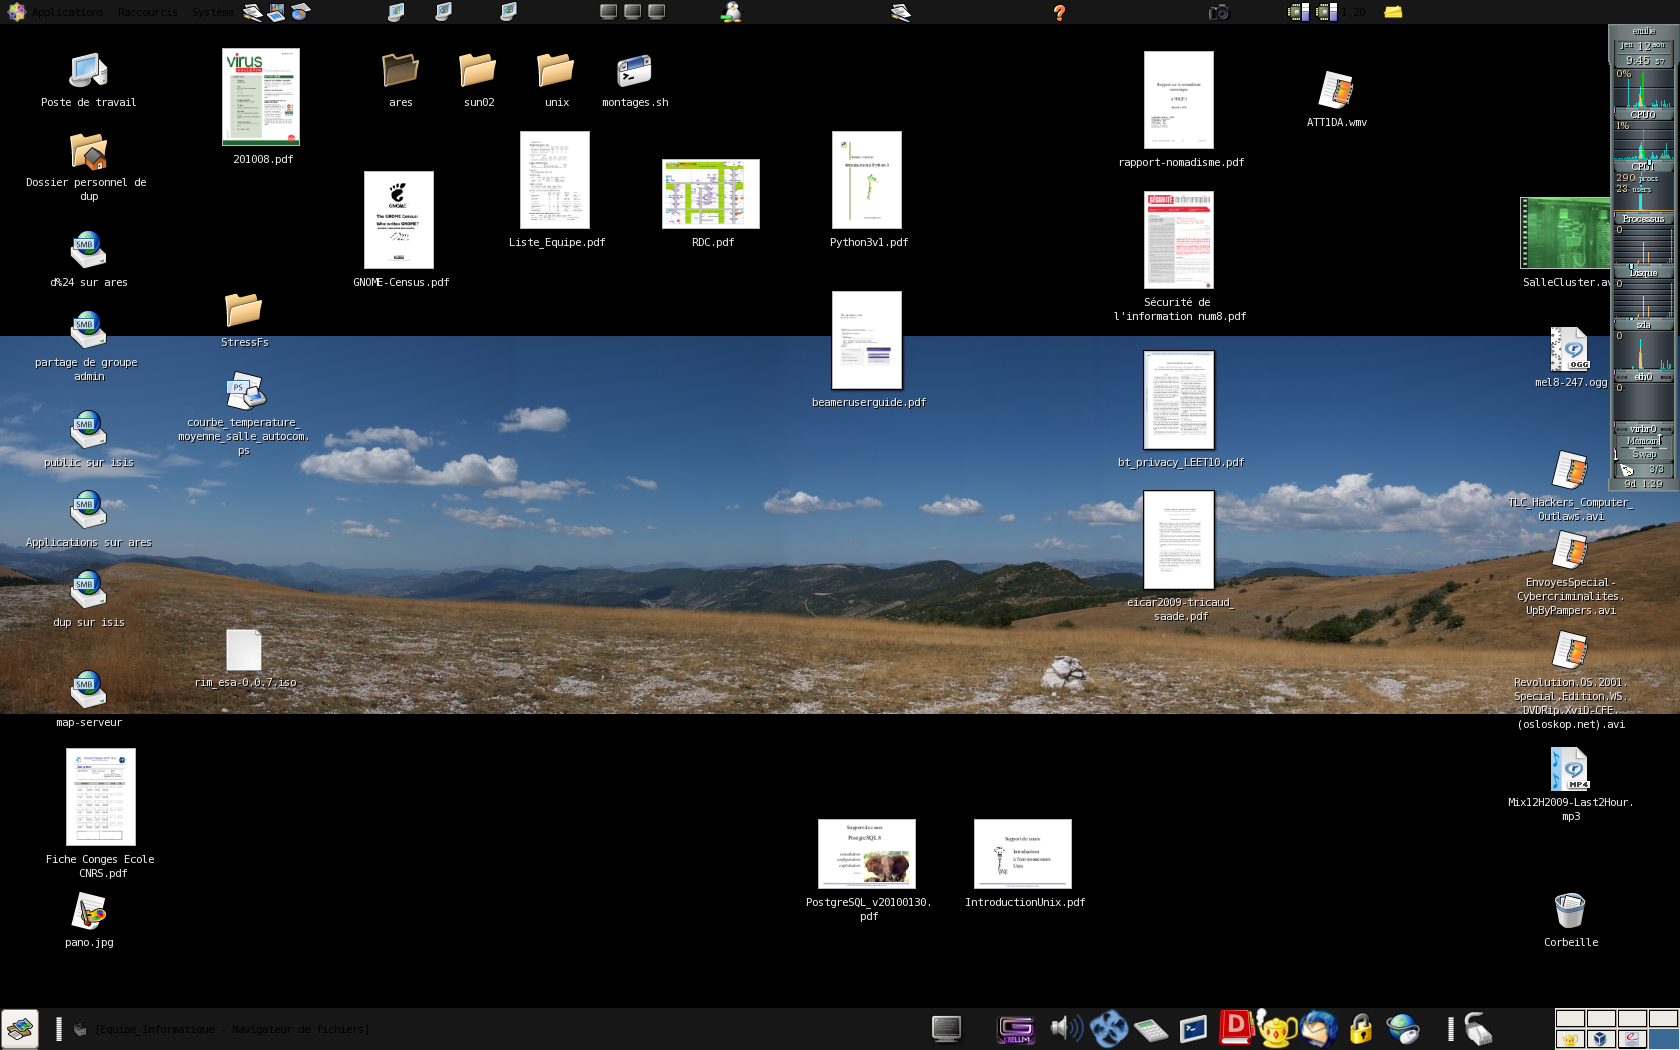
\includegraphics[width=9cm]{images/ecran.png}
            \caption{Environnement graphique}
        \end{figure}

    \end{center}
}


\frame
{
    \frametitle{Quel environnement aujourd'hui}

     \begin{center}

        \begin{figure}
            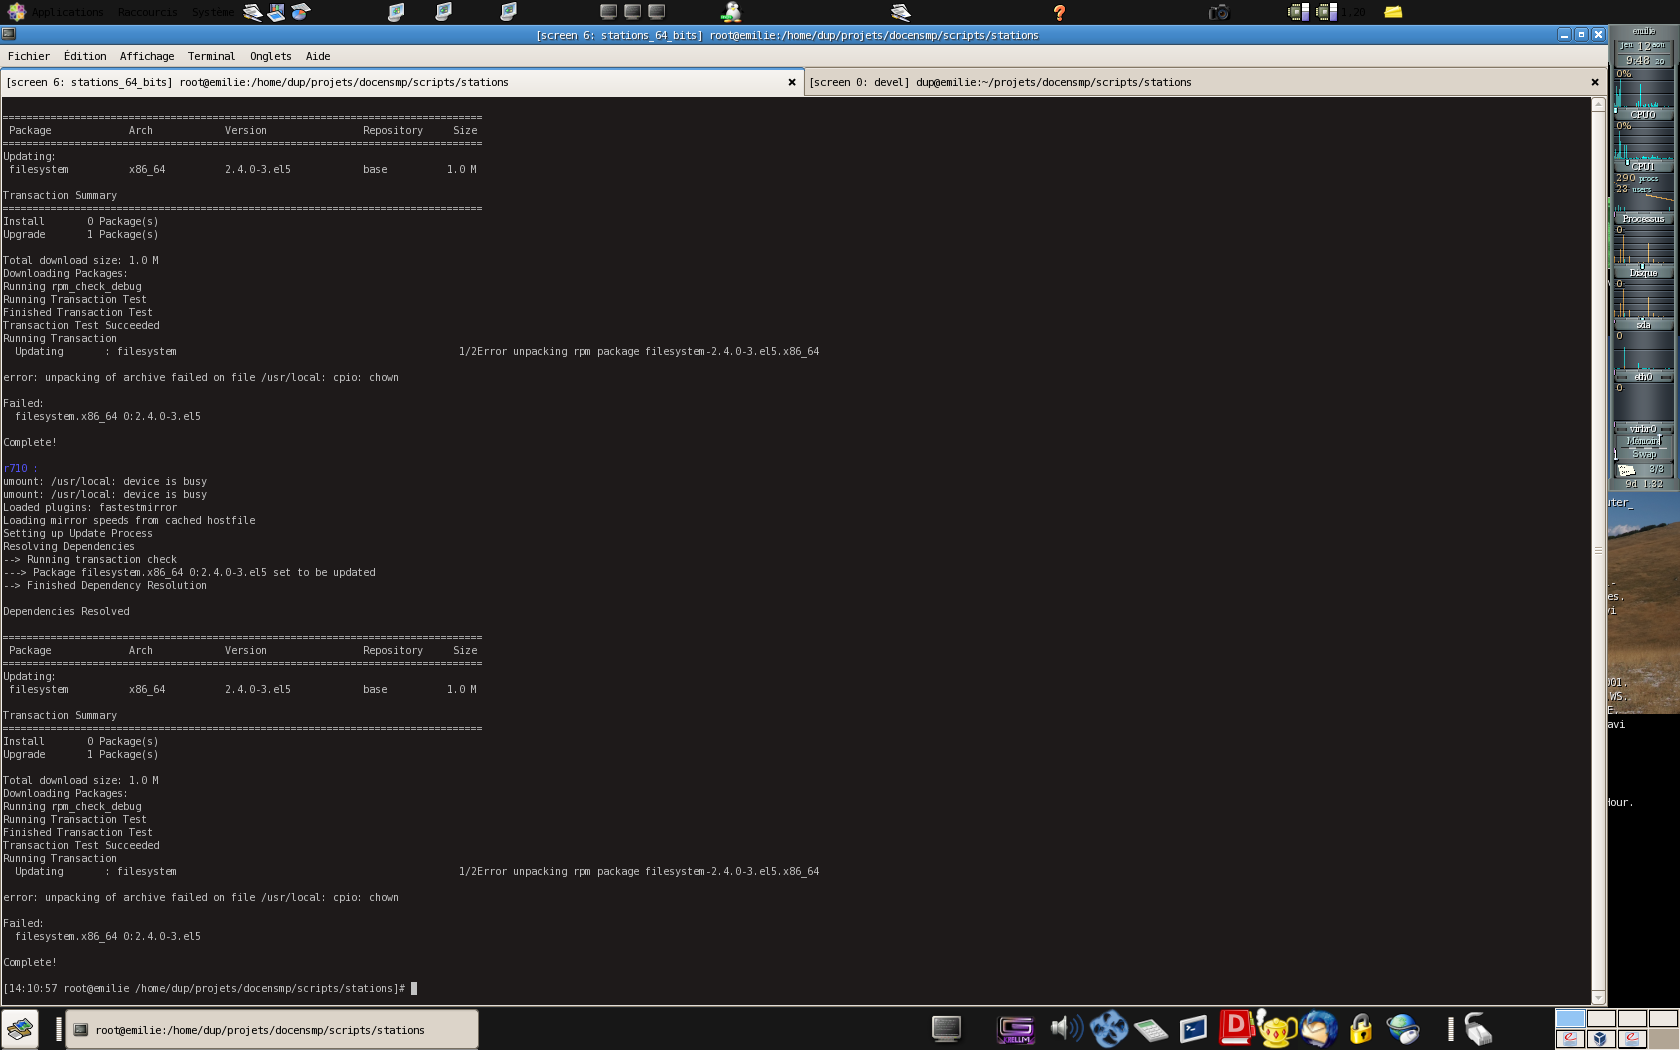
\includegraphics[width=9cm]{images/ligne_commande.png}
            \caption{Ligne de commande}
        \end{figure}

    \end{center}
}


\frame
{
    \frametitle{Trucs et astuces (clavier et souris)}

    \begin{exampleblock}{\textit{Astuces diverses}}
        \begin{itemize}
            \item La touche majuscule permet de faire les majuscules accentuées ÉÈÀÛ...,
            \item La sélection avec la souris puis le clic du bouton du milieu réalise un copier/coller,
            \item L'appui sur la touche <<chapeau>> puis sur un chiffre (hors pavé numérique) permet de faire un exposant : $ \mathnormal{^{123456789}}. $
        \end{itemize}
    \end{exampleblock}
}


\section{La ligne de commande}
\frame
{
    \frametitle{Pourquoi la ligne de commande ?}

    \begin{itemize}
        \item Pas d'équivalent graphique aussi puissant,
        \item Mise en oeuvre immédiate,
        \item Le travail à distance est facilité (plus rapide qu'en graphique) et
              c'est parfois la seule façon d'accéder à un serveur (par exemple un
              serveur de calcul),
       % \item \textit{Tout est fichier !}
    \end{itemize}
}


\frame
{
    \frametitle{Présentation de la ligne de commande}

    \begin{itemize}
        \item Elle est formée par une invite de commande : {\ttfamily tp1.dup$\mathnormal{[31]}$\%}
            \begin{itemize}
                \item Cette invite de commande est modifiable,
                \item Ici il indique le nom de la machine et le nom de login et le numéro de la commande entre crochets,
                \item Elle est fournie par un program que l'on nomme le shell,
            \end{itemize}
        \item On peut saisir du texte et des commandes sur cette ligne comme par exemple {\ttfamily man}, {\ttfamily pwd}, {\ttfamily clear}.
    \end{itemize}
}


\frame
{
    \frametitle{Généralités sur les commandes}

    \begin{itemize}
        \item Une commande est formée ainsi : \textbf{commande} \textit{arguments}
            \begin{itemize}
                \item L'espace est un séparateur (entre la commande et les arguments et pour les arguments),
                \item Les arguments peuvent être optionnels,
                \item Les arguments peuvent êtres des options ou des noms de fichiers,
                \item Chaque commande a ses propres options,
                \item Les options courtes s'indiquent avec un seul - et les longues avec deux,
                \item Les options courtes peuvent s'additionner,
                \item \textcolor{red}{\textbf{Souvent les options \textit{-h}, \textit{--help} fournissent l'aide de la commande}},
                \item \textcolor{red}{\textbf{La commande {\ttfamily man} suivie du nom d'une commande donne l'aide de cette dernière.}},
                \item Un double - optionnel permet d'indiquer la fin des options.
            \end{itemize}
    \end{itemize}
}


\section{Système de fichiers}
\frame
{
    \frametitle{Arborescence}

    \begin{itemize}
        \item Il n'y a pas de lecteurs sous Linux / Unix,
        \item Tout est sous forme d'arbre dont les noeuds sont les dossiers et les feuilles les fichiers,
        \item Un nouveau <<lecteur>> est <<raccroché>> sur un dossier.
        \item Les dossiers {\ttfamily .} et {\ttfamily ..} sont spéciaux et présents dans tous les dossiers.
    \end{itemize}
}


\frame
{
    \frametitle{L'arborescence du système de fichier}

    \begin{center}

        \begin{figure}
            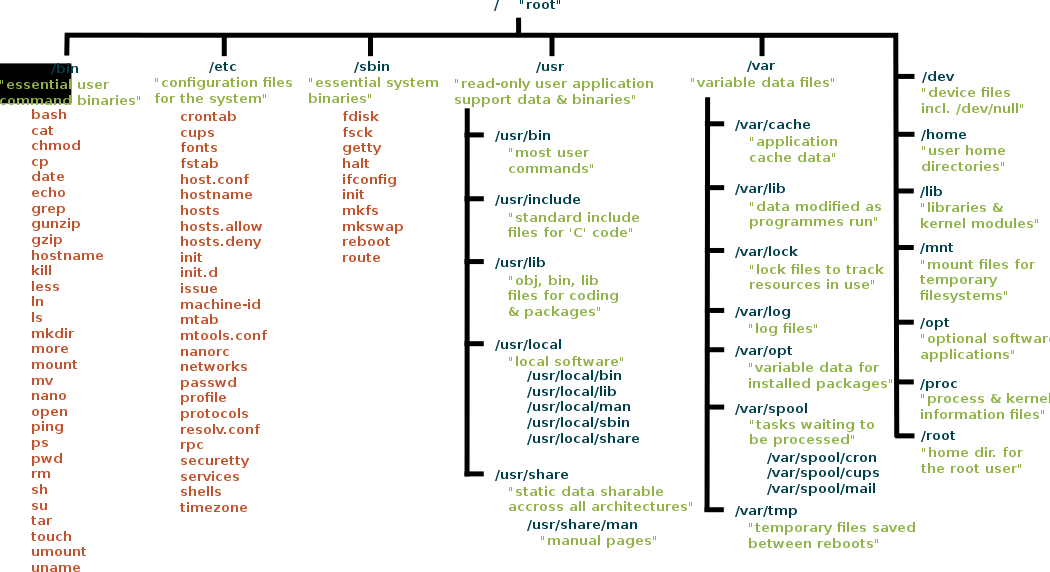
\includegraphics[height=6cm]{images/Standard-unix-filesystem-hierarchy.png}
            \caption{arborescence \tiny{(image issue de wikimedia - Ppgardne CC-BY-SA 4.0)}}
        \end{figure}

    \end{center}
}


\frame
{
    \frametitle{Quelques commandes utiles pour se déplacer}

    \begin{itemize}
        \item {\ttfamily pwd} Indique de manière absolue où on se trouve dans l'arborescence,
        \item {\ttfamily cd} Permet de naviguer dans l'arborescence. {\ttfamily cd -} permet de revenir au dossier précédent.
    \end{itemize}

    Chemins relatifs et absolus :

    \begin{itemize}
        \item Il est possible de se déplacer de deux façons :
            \begin{itemize}
                \item De manière absolue (par rapport à la racine),
                \item De manière relative (par rapport à l'endroit où on se trouve dans l'arborescence),
            \end{itemize}
    \end{itemize}
}


\frame
{
    \frametitle{Une commande utile pour lister les fichiers et dossiers}

    \begin{itemize}
      \item {\ttfamily ls} Liste les fichiers et dossiers (tout est fichier !)
            \begin{itemize}
                \item option -d pour un dossier,
                \item option -a pour voir tous les fichiers y compris les cachés,
                \item option -t pour classer en fonction de la date (-r pour renverser l'ordre),
                \item option -s pour obtenir la taille en blocs,
                \item option -l pour voir plus de détails.
            \end{itemize}
      \item Exemples :
            \begin{itemize}
                \item {\ttfamily ls -l -a}
                \item {\ttfamily ls -lart}
            \end{itemize}
    \end{itemize}
}


\frame
{
    \frametitle{Digression sur l'expansion des noms de fichiers}

    \begin{itemize}
        \item On peut utiliser des méta-caractères pour indiquer un raccourci ou un ensemble de fichiers
        \item Les méta-caractères :
            \begin{itemize}
                \item \tild
                \item *
                \item ?
                \item $\mathnormal{[~]}$
            \end{itemize}
    \end{itemize}
}


\frame
{
    \frametitle{Les fichiers, les dossiers et les droits associés}

    Exemples :

    \begin{itemize}
        \item {\ttfamily lrwxrwxrwx}
        \item {\ttfamily drwxr-xr-x}
        \item {\ttfamily -rw-r--r--}
    \end{itemize}

    1 lettre et 3 groupes de 3 lettres : {\ttfamily d rwx r-x r-x}

    \begin{itemize}
        \item le type de fichier (-, d, l, c, b, s),
        \item les droits sur le fichier en fonction du groupe (utilisateur, groupe, tous les autres).
    \end{itemize}

    \begin{itemize}
        \item 'r' indique un droit de lecture,
        \item 'w' indique un droit d'écriture,
        \item 'x' indique un droit d'exécution.
    \end{itemize}
}


\frame
{
    \frametitle{Changer les droits}

    \begin{itemize}
        \item la commande est {\ttfamily chmod} pour 'change mode',
        \item les lettres 'u', 'g' et 'o' indiquent respectivement l'utilisateur, le groupe et les autres,
        \item '+' pour ajouter des droits et '-' pour enlever des droits,
        \item on peut indiquer l'ensemble des droits avec la notation modale.
    \end{itemize}

    Exemples :

    \begin{itemize}
        \item {\ttfamily chmod o+r monfichier},
        \item {\ttfamily chmod g+w monfichier},
        \item {\ttfamily chmod go-rx monfichier}.
    \end{itemize}
}


\frame
{
    \frametitle{Changer le propiétaire}

    \begin{itemize}
        \item la commande est {\ttfamily chown} pour 'change owner',
        \item on indique le nouveau propriétaire (éventuellement le groupe) et les fichiers auxquels cela s'applique,
        \item l'option '-R' permet de faire les changements récursivement (pour toute une arborescence),
        \item la commmande {\ttfamily chgrp} permet de ne changer que le groupe.
    \end{itemize}

    Exemples :

    \NoAutoSpaceBeforeFDP
    \begin{itemize}
        \item {\ttfamily chown dup monfichier}
        \item {\ttfamily chown dup:admin monfichier}
        \item {\ttfamily chown -R dup:admin mondossier}
        \item {\ttfamily chgrp -R admin monautredossier}
    \end{itemize}
    \AutoSpaceBeforeFDP
}


\frame
{
    \frametitle{Recherche un fichier en fonction de critères externes}

    \begin{itemize}
        \item '{\ttfamily find nomdudossier options}' permet de rechercher (récursivement) des fichiers en fonction de critères externes.
            \begin{itemize}
                \item '-type' pour rechercher des fichiers d'un certain type (f pour fichier, d pour dossier, l pour lien),
                \item '-size n' fichier dont la taille est au moins n,
                \item '-perm -g=rx' en fonction des droits sur les fichiers (ici lecture et exécution au groupe),
                \item '-user u' les fichiers doivent appartenir à l'utilisateur u,
                \item '-group g' les fichiers qui appartiennent au groupe g,
                \item '-exec action' exécute l'action sur chacun des fichiers trouvés.
            \end{itemize}
    \end{itemize}

    Exemples :

    \begin{itemize}
        \item {\ttfamily find /etc -type d -perm -o=rx}
        \item {\ttfamily find /etc -type f -size 4k -exec cat \{\} $\setminus$;}
    \end{itemize}
}


\frame
{
    \frametitle{Commandes pour travailler avec des fichiers (1/11)}

    \begin{itemize}
        \item {\ttfamily cp src dst} pour 'copy' :
            \begin{itemize}
                \item copie un fichier ou des fichiers,
                \item option '-r' (récursif) pour la copie d'un dossier et de ses sous dossiers,
                \item option '-p' (préserve) pour préserver les droits,
                \item option '-a' (archive) pour copier tout tel quel sans changements.
            \end{itemize}
        \item {\ttfamily mv src dst} pour 'move' :
            \begin{itemize}
                \item déplace ou renomme un fichier ou un dossier.
            \end{itemize}
        \item {\ttfamily mkdir nomdudossier} pour 'make directory' :
            \begin{itemize}
                \item Une option possible est l'option '-p' (parents) qui demande la création des dossiers parents s'ils n'existent pas.
            \end{itemize}
    \end{itemize}

    \textit{'{\ttfamily dst}' peut être un dossier ou un fichier. Il peut y avoir plusieurs sources mais qu'une seule destination !}
}


\frame
{
    \frametitle{Commandes pour travailler avec des fichiers (2/11)}

    \begin{itemize}
        \item {\ttfamily rm nomfichier} pour 'remove' :
            \begin{itemize}
                \item détruit un fichier (ou un dossier),
                \item option '-r' pour supprimer des dossiers (attention la commande est récursive).
            \end{itemize}
        \item {\ttfamily rmdir nomdossier} pour 'remove directory' soit détruire un dossier.
    \end{itemize}

    \begin{alertblock}{Attention}
        La suppression via ces commandes est définitive (il n'y a pas de dossier <<Poubelle>>).
    \end{alertblock}
}


\frame
{
    \frametitle{Commandes pour travailler avec des fichiers (3/11)}

     \begin{itemize}
        \item {\ttfamily file nomfichier} pour connaitre le type du fichier en fonction de son contenu,
        \item {\ttfamily cat nomfichier1 nomfichier2} pour afficher ou concatener des fichiers,
        \item {\ttfamily grep PATRON nomfichier} permet de rechercher PATRON dans un fichier et d'en afficher les correspondances.
            \begin{itemize}
                \item '-E' pour utiliser les expressions rationnelles étendues,
                \item '-r' permet d'effectuer une recherche récursive (dans les sous-dossiers),
                \item '-i' ne pas tenir compte de la casse (majuscules/minuscules),
                \item '-l' afficher le nom du fichier plutôt que la correspondance.
            \end{itemize}
    \end{itemize}
}


\frame
{
    \frametitle{Digressions sur les expressions rationnelles (1/2))}

    Une expression rationnelle c'est un patron, c'est à dire un modèle qui décrit une suite de caractère formant une chaine de caractère.

    \begin{itemize}
        \item {\ttfamily |} indique un choix : essai|test,
        \item {\ttfamily .} indique n'importe quel caractère,
        \item {\ttfamily ?} défini un groupe qui existe 0 ou une fois,
        \item {\ttfamily *} défini un groupe qui existe 0 ou n fois,
        \item {\ttfamily +} défini un groupe qui existe 1 ou n fois,
        \item {\ttfamily \circonflexe} recherche une correspondance en début de ligne,
        \item {\ttfamily \$} recherche une correspondance en fin de ligne,
        \item {\ttfamily [~]} défini une classe de caractère,
        \item {\ttfamily [\circonflexe ~]} défini le complément de la classe de caractère,
        \item {\ttfamily \{m,n\}} défini au moins m correspondances et au plus n.
    \end{itemize}
}


\frame
{
    \frametitle{Digressions sur les expressions rationnelles (2/2))}

    Exemples :

    \begin{itemize}
        \item {\ttfamily [cC]hat|[cC]hien} : chat ou Chat ou chien ou Chien (grep -i -E 'new|conf' /etc/*),
        \item {\ttfamily chu+t} chut ou chuut ou chuuuuuut, etc ...,
        \item {\ttfamily peu[xt]?} Les mots qui contiennent peu ou peux ou peut,
        \item {\ttfamily \circonflexe trax\$} correspond aux lignes qui ne comportent que le mot trax,
        \item {\ttfamily c[o]?nf\$} cnf ou conf en fin de ligne (grep -i -E 'new\$|conf\$' /etc/*),
        \item {\ttfamily se[a-Z]*es} les mots qui commencent par es et finnissent par se : sees, services, sevices, ...,
        \item {\ttfamily \circonflexe rc[\circonflexe a-Z]\{0,1\}$\backslash$.d} toutes les lignes qui commencent par "rc" qui ont, ou pas, un caractère qui n'est pas dans l'ensemble "a-Z" puis qui comporte un "." et un "d".
    \end{itemize}
}


\frame
{
    \frametitle{Commandes pour travailler avec des fichiers (4/11)}

    \begin{center}{\textbf{Tout est fichier !}} {\textit{(et flux)}}\end{center}

    \begin{itemize}
        \item Une commande est toujours connectée à 3 <<flux>> :
            \begin{itemize}
                \item \textcolor{green}{le flux d'entrée (stdin)   (descripteur de fichier 0)},
                \item  \textcolor{blue}{le flux de sortie (stdout) (descripteur de fichier 1),}
                \item \textcolor{red}{le flux d'erreurs (stderr) (descripteur de fichier 2)},
            \end{itemize}
        \item On peut rediriger les flux avec les signes {\ttfamily >} et {\ttfamily <} :
            \begin{itemize}
                \item {\ttfamily >} redirige le flux de sortie vers un fichier (écrase le fichier),
                \item {\ttfamily >>} redirige le flux de sortie vers un fichier (concatène à la suite),
                \item {\ttfamily <} redirige le flux d'un fichier vers l'entrée de la commande,
            \end{itemize}
    \end{itemize}
}


\frame
{
    \frametitle{Commandes pour travailler avec des fichiers (5/11)}

    \begin{itemize}
        \item le pipe '{\ttfamily |}' (AltGr-6) ou tube permet de passer un flux d'une commande à l'autre
              (pour chainer les commandes). C'est à dire passer le flux de sortie de la première commande
              au flux d'entrée de la seconde commande :
            \begin{itemize}
                \item  {\ttfamily cat nomfichier | grep essai}
            \end{itemize}
        \item {\ttfamily wc} permet de compter le nombre de lignes, de mots et de caractères dans un fichier :
            \begin{itemize}
                \item  {\ttfamily cat nomfichier | grep essai | wc -l}
            \end{itemize}
    \end{itemize}
}


\frame
{
    \frametitle{Commandes pour travailler avec des fichiers (6/11)}

    Voir le début ou la fin d'un fichier :

    \begin{itemize}
        \item {\ttfamily head}
        \item {\ttfamily tail}
    \end{itemize}

    \begin{itemize}
        \item option -n pour indiquer un nombre de ligne (head et tail),
        \item option -f pour indiquer à tail de ne pas quitter et de suivre les
              ajouts dans la fin du fichier.
    \end{itemize}

    Voir le contenu de fichiers trop longs (commandes interactives) :

    \begin{itemize}
        \item {\ttfamily more}
        \item {\ttfamily less}
        \item {\ttfamily most}
    \end{itemize}

    Exemple : {\ttfamily ls -ls /dev | less}
}


\frame
{
    \frametitle{Commandes pour travailler avec des fichiers (7/11)}

    \begin{itemize}
        \item {\ttfamily cut} pour n'afficher que certains champs d'un fichier,
        \item {\ttfamily sed} pour traiter, à la volée, un flux (voir le man !).
    \end{itemize}

    Exemples :

    \begin{itemize}
        \item {\ttfamily cat /etc/passwd | cut -d'\string:' -f1,3,4},
        \item {\ttfamily ls -ls /etc/sysconfig/ | sed -n 1\tild 2p},
        \item {\ttfamily ls -ls /etc/sysconfig/ | sed -e s/d/Y/g}.
    \end{itemize}

    Référence :

    \begin{itemize}
        \item Pour sed : \href{http://www.grymoire.com/Unix/Sed.html}{http://www.grymoire.com/Unix/Sed.html}.
    \end{itemize}
}


\frame
{
    \frametitle{Commandes pour travailler avec des fichiers (8/11)}

    \begin{itemize}
        \item {\ttfamily sort} pour trier le contenu des fichiers.
            \begin{itemize}
                \item option '-k' pour indiquer le champ qui servira de clef de tri,
                \item option '-n' pour indiquer un tri numérique,
                \item option '-t' pour indiquer le séparateur de champ (l'espace par défaut),
                \item option '-r' pour renverser l'ordre du tri.
            \end{itemize}
    \end{itemize}
}


\frame
{
    \frametitle{Commandes pour travailler avec des fichiers (9/11)}

    Les fichiers compressés et les fichiers archives :

    \begin{itemize}
        \item {\ttfamily gzip}, {\ttfamily bzip2}, {\ttfamily xz} ou {\ttfamily pigz} compressent un fichier,
        \item {\ttfamily gunzip}, {\ttfamily bunzip2}, {\ttfamily unxz} ou {\ttfamily unpigz} décompressent un fichier,
        \item {\ttfamily tar} créé une archive (option 'c') ou extrait les fichiers d'une archive (option 'x').
    \end{itemize}

    \begin{itemize}
        \item {\ttfamily tar zcvf desktop.tar.gz ~/Desktop}
        \item {\ttfamily gunzip desktop.tar.gz}
        \item {\ttfamily bzip2 desktop.tar}
    \end{itemize}
}


\frame
{
    \frametitle{Commandes pour travailler avec des fichiers (10/11)}

    \begin{itemize}
        \item {\ttfamily uniq} pour supprimer (ou garder) les lignes en doublons.
            \begin{itemize}
                \item sans option affiche une seule fois les lignes en doublons,
                \item option '-u' pour n'afficher que les lignes uniques (n'affiche plus celles en doublons),
                \item option '-d' pour n'afficher que les lignes dupliquées.
            \end{itemize}
        \item {\ttfamily diff} affiche les différences entre deux fichiers
        \item {\ttfamily join} pour effectuer une jointure entre deux fichiers (il faut qu'il y ait un champ commun),
        \item {\ttfamily comm} pour afficher les lignes communes entre deux fichiers triés.
    \end{itemize}
}


\frame
{
    \frametitle{Commandes pour travailler avec des fichiers (11/11)}

    Pour aller plus loin vous pouvez aussi regarder le manuel ('man') des commandes suivantes :

    \begin{itemize}
        \item {\ttfamily tee} dupliquer la sortie,
        \item {\ttfamily fold} justifier le texte,
        \item {\ttfamily fmt} justifier sur une taille maximale (pas de découpe des mots),
        \item {\ttfamily tr} transliterer,
        \item {\ttfamily split} découper des fichiers en morceaux,
        \item {\ttfamily awk} travailler les fichiers en mode colonne (et non ligne),
        \item {\ttfamily rev} renverser le texte,
        \item {\ttfamily ln} créer un lien.
    \end{itemize}
}


\frame
{
    \frametitle{Commandes pour connaitre la place occupée / libre}

    \begin{itemize}
        \item {\ttfamily du} pour 'disk usage' donne la taille des fichiers (la place occupée par un ensemble de fichier ou de dossier). Appliquée à un dossier la commande est récursive et donne la taille de tous les fichiers et sous-dossiers (les options intéressantes sont -s et -h),
        \item {\ttfamily df} pour 'disk free' indique la place occupée et libre des disques connectés à la machine,
        \item {\ttfamily quota} indique vos quotas : place occupée, place maximale éventuellement temps restant avant blocage (l'option -s permet une meilleure lecture).
    \end{itemize}

    \textit{Rappel : ne pas débrancher directement les disques et clefs USB, les <<démonter>> correctement avec l'aide du navigateur.}
}


\section{Utilisateur}
\frame
{
    \frametitle{Identification}

    Chaque utilisateur a un identifiant unique dans le système c'est l'UID (User IDentification). De même chaque groupe a son identifiant ou GID (Group IDentification).

    \begin{itemize}
        \item {\ttfamily id} donne les informations de l'utilisateur, son nom, les groupes auxquels il appartient (avec les identifiants numériques),
        \item {\ttfamily whoami} ne donne que mon identifiant,
        \item {\ttfamily who} ou {\ttfamily w} donne la liste des utilisateurs connectés à la machine (w donne plus d'informations),
        \item {\ttfamily groups} indique les groupes de l'utilisateur,
        \item {\ttfamily finger} Permet d'obtenir le nom des personnes (et pas seulement le login),
        \item Associée à un nom elle donne plus d'informations. Fichiers {\ttfamily .plan} et {\ttfamily .project}.
    \end{itemize}
}


\section{Système}
\frame
{
    \frametitle{Le système}

    \begin{itemize}

        \item {\ttfamily uname} avec l'option {\ttfamily -a} donne l'ensemble des informations système,
        \item Les fichiers {\ttfamily /proc/cpuinfo} et {\ttfamily /proc/meminfo} donnent des informations sur les CPU et la mémoire.
    \end{itemize}
}


\section{Processus}
\frame
{
    \frametitle{Un processus ? (1/2)}

    \begin{itemize}
        \item Il s'agit d'un programme en cours d'exécution (ou pas),
        \item Chaque commande qui est lancée est un processus (ou un ensemble de processus),
        \item La ligne de commande elle même est un processus (tcsh chez nous),
        \item Le système lui même est géré par un ensemble de processus.
    \end{itemize}
}


\frame
{
    \frametitle{Un processus ? (2/2)}

    \begin{itemize}
        \item Chaque processus a un numéro (PID - Process IDentification),
        \item Chaque processus a un processus père (PPID - Parent Process IDentification). Leur père à tous est numéro 1,
        \item Pour chaque processus le système attribue une priorité (modifiable à la baisse).
    \end{itemize}
}


\frame
{
    \frametitle{Voir les processus}

    Il existe plusieurs commandes :

    \begin{itemize}
        \item {\ttfamily ps} Il existe des tas d'options et de variantes pour {\ttfamily ps}. Quelques options utiles sous Linux sont :
            \begin{itemize}
                \item '-e' pour avoir tous les processus,
                \item '-f' pour avoir l'ensemble des paramètres (full) avec notamment la ligne de commande entière du processus,
                \item '-l' pour avoir une sortie complète (longue) et non tronquée,
                \item 'f'  (sans le -) donne l'arborescence des processus,
            \end{itemize}
        \item {\ttfamily top} et {\ttfamily htop} sont des programmes interactifs où l'on voit l'évolution des processus en temps (presque) réel.
    \end{itemize}
}


\frame
{
    \frametitle{Voir les processus - un exemple de ps}

    \includegraphics[width=10.5cm]{images/ps_image.png}
}


\frame
{
    \frametitle{Voir les processus - un exemple de htop}

    \includegraphics[width=10.5cm]{images/exemple_htop.png}
}


\frame
{
    \frametitle{Repérer la charge de la machine avec top ou htop}

    Par charge (load) on entend le taux d'occupation ou d'utilisation.

    \begin{itemize}
        \item load average : la moyenne à 1 minute, 5 minutes et 15 minutes de programmes fonctionnant à 100\%,
        \item occupation mémoire : totale, libre, utilisée et en cache (+swap),
        \item occupation processeur avec top,
        \begin{itemize}
            \item us = user (les programmes utilisateurs),
            \item sys = système (le sytème),
            \item wa = iowait (les entrées sorties en attente de traitement),
            \item id = idle (quand le processeur ne fait rien).
        \end{itemize}
        \item occupation processeur avec htop :
        \begin{itemize}
            \item regarder les barres horizontales qui indiquent le taux d'occupation de chaque processeur (ou coeur).
        \end{itemize}
    \end{itemize}
}


\frame
{
    \frametitle{Lancer un processus régulièrement}

    \begin{itemize}
        \item {\ttfamily watch} lance un processus (toutes les 2 secondes) et affiche sa sortie.
    \end{itemize}

    Suivi visuel de la modification de la liste des fichiers d'un dossier (création ou suppression de fichiers) :

    \begin{itemize}
        \item {\ttfamily watch -n 10 ls -ls mondossier}.
    \end{itemize}
}


\frame
{
    \frametitle{Lancer des processus en arrière plan}

    Jusqu'à présent on lance le processus et on attend qu'il se termine mais on peut lancer des processus longs en arrière plan :

    \begin{itemize}
        \item {\ttfamily \&} - Mis après une commande : {\ttfamily xeyes \&},
        \item  Pour vérifier les processus en cours utilisez la commande {\ttfamily jobs},
        \item {\ttfamily Ctrl-Z} arrête le processus en avant plan,
        \item {\ttfamily bg} (pour background) met un processus arreté en arrière plan,
        \item {\ttfamily fg} (pour foreground) ramène un processus de l'arrière plan en avant plan,
        \item {\ttfamily nice} et {\ttfamily renice} permettent la modification de la priorité.
    \end{itemize}
}


\frame
{
    \frametitle{Tuer un ou des processus}

    Vous ne pouvez tuer que les processus qui vous appartiennent !

    \begin{itemize}
        \item {\ttfamily kill PID} tue le processus numéro PID,
        \item {\ttfamily pkill} comporte plus d'options permettant de filtrer les processus,
        \item {\ttfamily killall nomduprocessus} tue tous les processus nommés 'nomduprocessus'.
    \end{itemize}
}


\section{Connexion à d'autres machines}
\frame
{
    \frametitle{ssh (secure shell)}

    Permet de se connecter sur une machine distante :

    \begin{itemize}
        \item {\ttfamily ssh nomdelamachine},
        \item {\ttfamily -X} permet de transférer l'affichage graphique (X11),
        \item {\ttfamily hostname} donne le nom de la machine sur laquelle on est connecté.
    \end{itemize}
}


\frame
{
    \frametitle{scp : copier des fichiers d'une machine à l'autre}

    Permet de copier des fichiers d'une machine sur une autre.

    \begin{itemize}
        \item {\ttfamily scp src dst},
        \item {\ttfamily -r} permet de copier récursivement un dossier,
        \item {\ttfamily -p} (pour preserve) préserve les permissions des fichiers lors de leur copie.
    \end{itemize}

    Exemple :
    \begin{itemize}
        \item {\ttfamily scp monfichier unemachine\string:/home/dup}
        \item {\ttfamily scp -rp unemachine\string:/home/dup machinedeux\string:/tmp}
    \end{itemize}
}


%\frame
%{
    %\frametitle{sftp : un système de transfert de fichiers entre deux machines}

    %Permet de transférer des fichiers entre deux machines

    %\begin{itemize}
        %\item {\ttfamily sftp utilisateur@nomdelamachine} se connecte à la machine distante et passe en mode interactif
        %\item {\ttfamily sftp utilisateur@nomdelamachine\string:/nomdudossier} démarre dans le dossier 'nomdudossier'
    %\end{itemize}
%}


%\frame
%{
    %\frametitle{sftp : un système de transfert de fichiers entre deux machines}

    %\begin{itemize}
        %\item Les commandes sont exécutées sur la machine distante (ls, cd, ...)
        %\item {\ttfamily !} placé devant une commande : exécute cette dernière sur la machine locale
        %\item {\ttfamily get nomdufichier} récupère 'nomdufichier' de la machine distante vers la machine locale
        %\item {\ttfamily put nomdufichier2} envoi 'nomdufichier2' de la machine locale vers la machine distante
        %\item {\ttfamily ?} donne l'aide
        %\item {\ttfamily quit} quitte sftp
    %\end{itemize}
%}


% Unix avancé :
% - les signaux
% - les variables d'environnement
% - substitution de commandes : $() ou ``
% - création de scripts
%


\section{Unix avancé}
\frame
{
    \frametitle{Les signaux (1/2)}

    Les programmes peuvent envoyer et/ou recevoir des signaux. On utilise ce mécanisme sans le savoir :
    Lorsque l'on tape Ctrl-Z ou Ctrl-C le système envoi un signal au processus.
    Il s'agit de STOP (Ctrl-Z) et INT (Ctrl-C).

    \begin{itemize}
        \item {\ttfamily kill} est la commande qui permet d'envoyer des signaux (avec l'option {\ttfamily -s}). Par défaut elle envoie le signal {\ttfamily TERM},
        \item {\ttfamily kill -l} donne la liste des signaux que l'on peut envoyer,
        \item Les signaux {\ttfamily STOP} et {\ttfamily KILL} ne peuvent ni être ignorés ni interceptés par un processus.
    \end{itemize}

    Exemple avec la commande {\ttfamily dd if=/dev/zero of=/dev/null} et le signal {\ttfamily USR1}.
}


\frame
{
    \frametitle{Les signaux (2/2)}

    Les signaux les plus usités sont :

    \begin{itemize}
        \item {\ttfamily STOP} qui stoppe l'exécution du processus,
        \item {\ttfamily CONT} qui reprend l'exécution d'un processus arrêté,
        \item {\ttfamily TERM} qui demande (poliment) au processus de se terminer,
        \item {\ttfamily KILL} qui termine le processus (il n'a pas le choix !),
        \item {\ttfamily USR1} qui est utilisé pour implémenter un signal spécifique à l'application.
    \end{itemize}
}


\frame
{
    \frametitle{Les alias de commandes}

    La commande {\ttfamily alias} permet de définir un alias pour une commande ({\ttfamily unalias} pour faire l'inverse)

    Quelques exemples :

     \begin{itemize}
        \item {\ttfamily alias} : sans argument donne la liste de tous les alias existants,
        \item {\ttfamily alias dir ls -ls} : taper dir dans la ligne de commande exécute {\ttfamily ls -ls},
        \item {\ttfamily alias ll ls -ls | less}  : la même chose mais avec un tube et l'exécution de  {\ttfamily less}.
%        \item {\ttfamily alias zset=unsetenv NEWZ7PATH; if ( -d !* ) setenv NEWZ7PATH !*; \\
%            if ( ! \$?NEWZ7PATH ) setenv NEWZ7PATH /home/zebulon/!*; $\backslash$
%            if ( -d \$NEWZ7PATH ) setenv Z7PATH \$NEWZ7PATH ; $\backslash$
%             source \$Z7PATH/lib/Z7cshrc ; $\backslash$
%            unsetenv NEWZ7PATH}
    \end{itemize}
}


\frame
{
    \frametitle{Les variables d'environnement}

    Il s'agit de variables que l'on peut fixer dans le shell. C'est très utile pour
    modifier un comportement seulement dans un shell donné (et de manière temporaire).

    \begin{itemize}
        \item par convention notées en majuscules.
        \item Les variables d'environnement peuvent être utilisées avec les commandes ou les alias de commandes.
    \end{itemize}
}


\frame
{
    \frametitle{Les variables d'environnement en tcsh}

    \begin{itemize}
        \item {\ttfamily setenv} : liste toutes les variables d'environnement (chemins, options de compilation, ...),
        \item {\ttfamily setenv TPPATH /home/users/dup/TP} : affecte {\ttfamily /home/users/dup/TP} à la variable d'environnement {\ttfamily TPPATH},
        \item {\ttfamily \$} placé devant le nom d'une variable d'environnement pour y faire référence : {\ttfamily echo \$TPPATH},
        \item {\ttfamily unsetenv TPPATH} supprime la variable d'environnement {\ttfamily TPPATH}.
    \end{itemize}
}


\frame
{
    \frametitle{La commande module}

    ... ou la manipulation des variables d'environnement sans y penser ...

    \begin{itemize}
        \item {\ttfamily module list} Liste les modules chargés
        \item {\ttfamily module avail} Liste les modules disponibles
        \item {\ttfamily module load unmodule} Charge un module
        \item {\ttfamily module unload unmodule} Décharge un module
    \end{itemize}
}


\frame
{
    \frametitle{La substition de commande}

    On peut inclure une commande dans une autre en utilisant les côtes obliques (AltGr-7) : `macommande`.

    Exemples :

    \begin{itemize}
        \item {\ttfamily echo -n `date -R`}
        \item {\ttfamily foreach i ( `ls` ) }\\ {\ttfamily ~~file \$i} \\ {\ttfamily ~~echo \$i} \\ {\ttfamily end}
        \item {\ttfamily setenv PWD `pwd`}
    \end{itemize}
}


\frame
{
    \frametitle{l'éditeur de fichier texte vim}

    Quatre modes sont couramment utilisés :

    \begin{itemize}
        \item mode normal (ou de déplacement) : dans ce mode taper {\ttfamily :help} pour avoir l'aide,
        \item mode d'édition : tapez {\ttfamily i} ou {\ttfamily a} pour entrer en mode édition, 
        \item mode commande : tapez {\ttfamily :} pour pouvoir entrer des commandes,
        \item mode sélection : tapez {\ttfamily v}, {\ttfamily V} ou encore {\ttfamily Ctrl+v}.
    \end{itemize}

    Quelque soit le mode, la touche <<Esc>> (ou <<Echap>>) permet de revenir au mode normal.

}


\frame
{
    \frametitle{l'éditeur de fichier texte vim}

    En mode normal (ou de déplacement) :

    \begin{itemize}
        \item {\ttfamily dd} pour supprimer une ligne,
        \item {\ttfamily x} pour supprimer un caractère,
        \item {\ttfamily u} pour undo,
        \item {\ttfamily p} pour coller le contenu du tampon mémoire,
        \item {\ttfamily G} va à la dernière ligne du fichier,
        \item {\ttfamily gg} va à la première ligne du fichier,
        \item {\ttfamily 1315} va à la ligne 1315.
    \end{itemize}
}


\frame
{
    \frametitle{l'éditeur de fichier texte vim}

    Le mode commande :
    
    \begin{itemize}
        \item {\ttfamily :} pour indiquer qu'une commande suit,
        \item commande {\ttfamily q} pour quitter (ajouter ! pour forcer),
        \item commande {\ttfamily w} pour sauvegarder (ajouter ! pour forcer).
    \end{itemize}

    On peut chainer les commandes et faire {\ttfamily :wq} pour sauvegarder et quitter.
}


\frame
{
    \frametitle{navigateur en mode texte}

    links :

    \begin{itemize}
        \item {\ttfamily links http://wikipedia.fr}
    \end{itemize}

    \begin{itemize}
        \item Les flèches du haut et du bas pour se balader dans la page,
        \item Les flèches droites et gauche pour aller et revenir dans l'historique,
        \item La touche 'd' pour télécharger, la touche 'q' pour quitter.
    \end{itemize}
}


\frame
{
    \frametitle{La création de scripts en tcsh}

    \begin{itemize}
        \item La première ligne indique le nom de l'interpréteur {\ttfamily \#!/bin/tcsh} pour ce qui nous concerne.
    \end{itemize}

    On trouve aussi (et des tas d'autres) :

    \begin{itemize}
        \item {\ttfamily \#!/usr/bin/perl}
        \item {\ttfamily \#!/usr/bin/env python}
        \item {\ttfamily \#!/bin/bash} ...
    \end{itemize}
}


\frame
{
    \frametitle{Paramètres des scripts (en tcsh)}

    \begin{itemize}
        \item {\ttfamily \$0} : le nom de du script
        \item {\ttfamily \$1, \$2, \$3}... les paramètres 1, 2, 3... du script ou de la fonction
        \item {\ttfamily \$*} : tous les paramètres
        \item {\ttfamily \$?} : le code de retour de la dernière commande
        \item {\ttfamily \$\$} : le numéro (PPID) du processus parent
        \item {\ttfamily \$!} : le numéro (PID) du dernier processus mis en tâche de fond
        \item {\ttfamily \$\_} : la dernière ligne de commande executée
    \end{itemize}

}


\frame
{
    \frametitle{Structures de contrôle (en tcsh)}

    \begin{itemize}
        \item {\ttfamily if (expression) then\dots else\dots endif}
        \item {\ttfamily switch (expression) case xy\string:\dots breaksw\dots case yx\string:\dots breaksw\dots endsw}
        \item {\ttfamily while (expression)\dots end}
        \item {\ttfamily foreach x (list)\dots end}
    \end{itemize}
}


\frame
{
    \frametitle{Exemples de structures de contrôle (1/2)}

    \begin{itemize}
        \item {\ttfamily foreach x (fichier1 fichier2) \\
                    ~~echo "\$x \string:" \\
                    ~~file \$x \\
                end\\
              }
        \item {\ttfamily switch (\$argv[1]) \\
                case -h\string:\\
                    ~~echo "Usage : exemple options args"\\
                    ~~breaksw\\
                case -t\string:\\
                case -T\string:\\
                    ~~file monfichier\\
                    ~~breaksw \\
                endsw\\
              }
    \end{itemize}
}


\frame
{
    \frametitle{Exemples de structures de contrôle (2/2)}

    \begin{itemize}
        \item {\ttfamily if (-e readme \&\& -r readme) then \\
                echo "Le fichier readme existe et est lisible"\\
                    ~~cat readme\\
                else if (-e readme)\\
                    ~~echo "Le fichier existe mais n'est pas lisible"\\
                else\\
                    ~~echo "Le fichier n'existe pas"\\
                endif\\
              }
        \item {\ttfamily set n=1\\
                while (\$n < 301)\\
                    ~~echo \$n\\
                    ~~@~n = (\$n + 1)\\
                    ~~@~n++\\
                end\\
              }
    \end{itemize}
}


\frame
{
    \frametitle{Opérateurs}

    \begin{itemize}
        \item Opérateurs logiques {\ttfamily ||  \&\&  }
        \item Opérateurs de comparaison de chaines {\ttfamily  == ~ != ~ =\tild ~ !\tild }
        \item Opérateurs de comparaison de nombres {\ttfamily <= ~  >= ~ < ~ > }
        \item Opérateurs arithmétiques {\ttfamily  |  \& ~ \circonflexe ~ + ~ - ~ * ~ / ~ \%  ~ ! ~ \tild ~ << ~ >> ~ ( ~ ) }
    \end{itemize}
}


\frame
{
    \frametitle{Opérateurs de tests sur les fichiers}

    Quelques opérateurs utiles :

    \begin{itemize}
        \item {\ttfamily -r}   Accès en lecture
        \item {\ttfamily -w}   Accès en écriture
        \item {\ttfamily -x}   Exécutable
        \item {\ttfamily -e}   Existence
        \item {\ttfamily -z}   Taille nulle
        \item {\ttfamily -s}   Taille non nulle
        \item {\ttfamily -f}   Fichier texte
        \item {\ttfamily -d}   Dossier
        \item {\ttfamily -l}   Lien symbolique
    \end{itemize}
}

\frame
{
    \frametitle{Merci !}

    Merci !

}


\end{document}
